\documentclass[pdftex,12pt,a4paper]{article}

\usepackage{amsmath}
\usepackage{graphicx}
\usepackage[usenames,dvipsnames]{xcolor}
\usepackage{tikz}
\usepackage[utf8]{inputenc}
\usepackage[english]{babel}
\usepackage{listings}
\usepackage{color}
\usetikzlibrary{calc}
\usetikzlibrary{decorations.pathmorphing}

\newcommand{\HRule}{\rule{\linewidth}{0.5mm}}
%\renewcommand{\thesection}{\arabic{section}} %Use this when using {report} document class and suffer 0.1 sectioning numbering
%\renewcommand{\baselinestretch}{1.5}

\definecolor{dkgreen}{rgb}{0,0.6,0}
\definecolor{gray}{rgb}{0.5,0.5,0.5}
\definecolor{mauve}{rgb}{0.58,0,0.82}

\lstset{frame=tb,
  language=C++,
  aboveskip=3mm,
  belowskip=3mm,
  showstringspaces=false,
  columns=flexible,
  basicstyle={\small\ttfamily},
  numbers=none,
  numberstyle=\tiny\color{gray},
  keywordstyle=\color{blue},
  commentstyle=\color{dkgreen},
  stringstyle=\color{mauve},
  breaklines=true,
  breakatwhitespace=true,
  tabsize=4,
  morekeywords={
  	sudo,
  	wget,
  	adv,
  	update,
  	install,
  	rosdep,
  	echo,
  	mkdir,
  	cd,
  	source,
  	catkin\_init\_workspace,
  	catkin\_make,
  	catkin\_create\_pkg,
  	rosnode,
  	rosservice,
  	rospack,
  	roscd,
  	rosls,
  	find\_package,
  	catkin\_package,
  	generate\_message,
  	add\_message\_files,
  	gzserver,
  	gzclient,
  	gazebo
  }
}

\pdfinfo {
			   /Title  (Robotic Arm Simulating Pre-Thesis)
               /Creator (Nguyen Vu Hoi)
               /Author (Nguyen Vu Hoi vuhoinguyen@gmail.com)
               /CreationDate (D:20030101000000)  %format D:YYYYMMDDhhmmss
               /ModDate (D:20030815213532)
               /Subject (Writing a Bachelor pre-thesis about simulation and controlling robotic arm)
               /Keywords (Bachelor, Thesis, Pre-thesis, Robotic, Arm, Gazebo, ROS, Robotics Operating System, Linux, Ubuntu, Vu Hoi Nguyen, VGU, Vietnamese-German University)}
                  
\begin{document}
  \begin{titlepage}
\begin{center}

% Upper part of the page. The '~' is needed because \\
% only works if a paragraph has started.

\includegraphics[width=0.3\textwidth]{./image/vgu_logo.png}~\\[1cm]
\textsc{\LARGE vietnamese-german university}~\\[0.2cm]
Electrical Engineering and Information Technology Department ~\\[3cm]
\textsc{\Large pre-thesis project}\\[0.5cm]

% Title
\HRule \\[0.4cm]
{ \huge \bfseries Robotic Arm:\\ Simulation on Linux \\ Using Gazebo and ROS \\[0.5cm] }

\HRule \\[3cm]

% Author and supervisor
\noindent
\begin{minipage}[t]{0.4\textwidth}
\begin{flushleft} \large
\emph{Author:}\\
Vu Hoi \textsc{NGUYEN}
\end{flushleft}
\end{minipage}%
\begin{minipage}[t]{0.4\textwidth}
\begin{flushright} \large
\emph{Supervisor:} \\
Prof. ~Peter \textsc{NAUTH} \\
Lab.Eng. Dinh Than \textsc{LE}
\end{flushright}
\end{minipage}
\vfill

% Bottom of the page
~\\[1cm]
{\large \today}

\end{center}

\begin{tikzpicture}[overlay,remember picture]

    \draw [line width=1mm,decorate,decoration={
        }]
        ($ (current page.north west) + (1cm,-1cm) $)
        rectangle
        ($ (current page.south east) + (-1cm,1cm) $);
        
\end{tikzpicture}

\end{titlepage}

  
  \pagenumbering{gobble}
  
  \newpage
  \tableofcontents
  \newpage
  \listoffigures
  
  \setlength{\parindent}{0em}
  \setlength{\parskip}{1em}
  
  \newpage
  \pagenumbering{arabic}
  \section*{Disclaimer}
  I declare that this report is a product of our own work, unless otherwise referenced. I also declare that all opinions, results, conclusions and recommendations are my own and may not represent the policies of opinions of the Vietnamese – German University.\\ \\ \\
  \begin{flushright}
  \textup{Nguyen Vu Hoi}
  \end{flushright}
  
  \newpage
  \section*{Abstract}
  This document is written as a requirement of the course "Elective project" for senior year in Vietnamese-German University. It reports the content of the project, my working process, the result and discuss the problems which are frequently occurs in the process.
  My project studies the controlling methods providing by Robotics Operating System (ROS) and simulation sequence using Gazebo on Linux (specifically distribution Ubuntu). \\
  The goal of the project is to successfully create a humanoid arm inside Gazebo and control its virtual joints using ROS.\par
  To do this, a virtual-physical model need to be coded using a marking language (xml). A robot is divided in to single "links" (ex. upper arm, forearm, hand, ...), connected by "joints" (ex. elbow, wrist, ...). These links are constructed by the simplest 3D shapes like spheres or boxes for faster and easier simulating. This model also holds the physical properties of the links such as dimensions of the parts, their mass, initials; type of the links (revolve, linear, ...) and relationship between the links and the joints. Gazebo then takes care of the relationships and simulate the behavior of the robot in the virtual environment.\par
  Furthermore, this model must have an appearance which is friendly to users (actual look of the robot, not just basic shapes). This "real" appearance is designed in another software, then exported (and imported into Gazebo) in form of a .stl file. Gazebo, again, take care of this change and display the new appearance of the robot into its 3D environment. \par
  As the last part, "virtual" motors are attached to the joints of the model and controlled by ROS. Although these joints can be controlled directly inside Gazebo, using ROS have a critical importance, as standardized ROS controlling methods can as well be used in other environments (including real life). That way, ROS will significantly reduce the future work if one attends to apply this simulation to a real robot, which is obviously the purpose in doing simulations and will be surely done.\par
  
  \newpage
  \section*{Acknowledgement}
  I would like to thank Mr. Nauth for his instruction and enthusiasm.\par
  I would like to thank Mr. Than for his help and explanation.\par
  I would like to thank Mr. Anis Koubaa for the tutorials and supports.\par
  And thank my classmates who gave me precious advice in working with an open-source project.
  
  \newpage
  \section{Introduction}
  \subsection{Simulation and its significance}
  Simulation means imitating the operation of a real-world process or system over time on the computer. The whole process of simulation often requires a virtual model. This model holds the key information and characteristics of the system in physical world. Using these information, we can have experiments in virtual world with similar result with that in real world. \par
  In my opinion, there are four main benefits in doing simulation before actual production of the robots.\\
  Firstly, the obvious advantage of this process is to reduce the cost of the failures. If a model is to be produced directly after design, there would be complications which are not yet available at that moment. These troubles can vary from mechanical problems, kinematic problems to usage problems. Using simulation, we can partially predict the problems and find solutions, or re-design them. In some cases, simulation plays a critical role. For example, to design robots which work on Mars. The environment may be harsh, too hot or too cold, strong or weak winds, along with thousands of other problems that are not available on Earth to experiment. Here came simulation, the tool that will minimize the risk of that robot. The more complex and ambitious the project is, the more important the simulation process is.\par
  Secondly, this virtual process increases the effectiveness of several developers in complex projects. For example, mechanical and software engineers can work independently. Software engineers don't have to wait for the actual robot to test their functions, and mechanical ones can have faster feedback about their design from their teammates. It also makes studying problems in different levels of abstraction available. In a complicated project, coders who write controlling functions (move motors, stabilize robot, ...) can work perfectly well without communicating engineers (with functions to communicate between parts of the robot). Simulation works as a solution of "cloning" as well, where every partner has their own "virtual robot" to test upon, while these robots are flawlessly synchronized by a single model.\par
  
  \newpage
  Expanding the benefit above, we get the third advantage of simulation: increased portability. A developer cannot work with the robot if the office is closed, or if some event needs its presence (demonstration, for example), or any reason which cuts their access to the robot. This problem is solved with a simulated model. He can improve his codes, write new functions, or re-design the robot at home, in coffee shop, or literally anywhere. This benefit is especially important to students, whose accessibility is often limited, and most comfortable place to work is in their rooms. \par
  \begin{figure}[h]
    \centering
    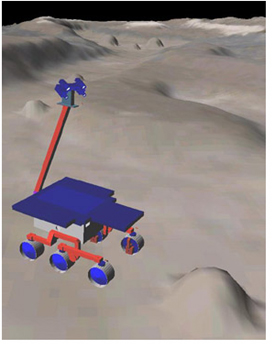
\includegraphics[width=0.5\linewidth]{image/107988main_Sim3.jpg}
    \caption{A rover robot simulated by NASA}
    \label{fig:nasa_robot}
  \end{figure}
  Fourthly, simulation makes it extremely easier to discuss upon, for teaching or demonstrating. By having a virtual model of the robot being your only requirement to show every of its aspects to people, discussing can never be faster and more convenient. If your boss tell you to show what functions have you written for the robot, you can show him visually just by turning your laptop on. If a friend has a great idea for a new way to solve the problem, you can test it immediately.\par
  With its importance, simulation is included in almost every robotic project. Therefore, this document hopefully helps anyone who concerns to find a simple way to make simulations on Linux.
  
  \newpage
  \subsection{Why Linux, ROS and Gazebo?}
  Linux is widely agreed to be the platform for robotics development. This statement is true mostly because of the large amount of supports available in Linux community.\\
  Since the beauty of robotics lies in linking the computer to physical world, Linux infrastructure provides many effective ways to communicate between devices. Most popular hardware and controller, for example Arduino, works very well with Linux. And the processing power of small microcomputers is increasing with a fantastic speed, making portable Linux devices a true thing. That way, the basic functions of robots can be programmed easily on this open-source platform. Moreover, the high quality community with a good knowledge of coding, whose philosophy is to help each other and make a better future with better technology, promote the development of this field dramatically. Therefore, more and more cutting-edge robotic projects are being built on Linux.\\
  Another important property of Linux is that it's free. You don't have to spend thousands of dollars for a software, can make as many robots with operating systems embedded in them as you want, and make experiments without worrying about a "wise investment". For a young university like Vietnamese-German University, I believe Linux is the most suitable researching platform of robotics field.\par
  \begin{figure}[h]
      \centering
      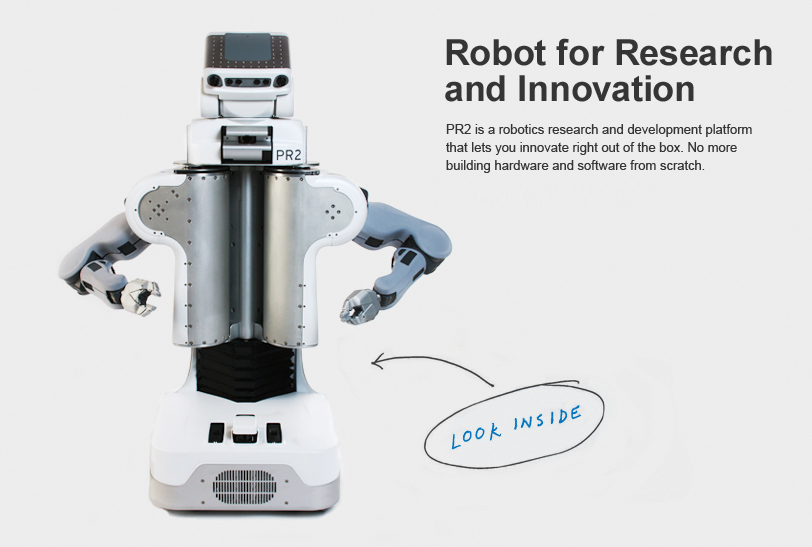
\includegraphics[width=0.8\linewidth]{image/pr2.jpg}
      \caption{PR2 - researching robot running primarily ROS}
      \label{fig:pr2_robot}
  \end{figure}
  However, the most important contributor to that success of Linux in robotics may be ROS. Robotics Operating System, ROS, was created in 2007 by Willow Garage company. Since then, it has unstoppably become one of the most powerful software environment for robotic development.\\
  On contrary to its name, ROS is not really an operating system. It is, in fact, a BSD-licensed open source software framework which runs on Linux. It provides standard  services such as package management, message-passing between processes, low-level device control, and implementation of common functionalities. These service simplifies the basic tasks of a developer, give them more time to concentrate on a specific research idea.\\
  ROS's influence is getting larger and larger. Many researchers and experts contributed to both ROS core ideas and its fundamental software packages, making starting learning robotics a much doable task for beginners like students.\\
  With ROS, a group can freely make their repository publicly available, receiving recognition and credit for their work. This also benefits them with technical feedbacks and improvements like any open-source project. However, they can also start their project on their own server, maintaining full ownership and control over that project. I think this feature is great for a research in a university. Vietnamese-German University can keep all their works on their own server, and publish only what they want.\\
  Therefore, for a newly started robotics department like VGU's, ROS may be the best choice. It's free, easy for students to study, and provide full control over the projects to the university. I personally have started using ROS for a short time, but realized the considerable potential of this platform.\par
  \begin{figure}[h]
      \centering
      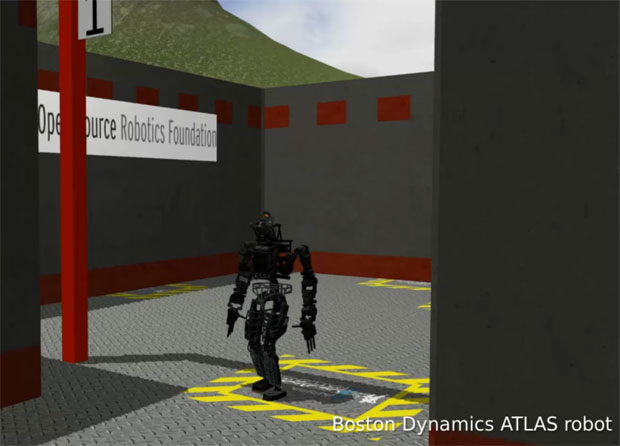
\includegraphics[width=0.65\linewidth]{image/drc_gazebo-1370245661467-1370270174909.jpg}
      \caption{A humanoid robot simulated in Gazebo}
      \label{fig:gazebo_sample}
  \end{figure}
  Lastly, the most important part of this project is the simulator: Gazebo.\\
  Gazebo was founded in 2002 at the University of Southern California. Its original aim was to simulate robots under various conditions in outdoor environment, as the name "gazebo" mean. However, through so many years with improvements, this tool can be used wonderfully in indoor environments.\\
  The highlight of Gazebo is its rich features. It provides accurate and fast simulation in complex environments, thanks to its robust physics engine. It offers advanced 3D graphics, where rendering is so realistic with all high quality textures, shadows and lighting. All kinds of sensors and noise, from contact sensor to Kinect's ones, can be generated optionally. Because of its strong support community, many robot models are available to be downloaded and experiment upon. Gazebo has cloud simulation and also works great with command line tools.\\
  That's why Gazebo has been one of the primary tools for ROS. It is compatible and works great with ROS. What is even better is a great community who support Gazebo, who also work with ROS. Tutorials are available with great details, and questions are answered enthusiastically.\\
  Although Gazebo also runs on Windows and Mac, Linux has always been the focus of its strategies.Therefore, if someone is about to start developing robotics with Linux and ROS, Gazebo is an essential tool to complete the combination.\par
  With all those reasons, Linux, along with ROS and Gazebo, should be choice for robotic researches in a new university like Vietnamese-German University. It offers a free entrance to the field, without trading off the potential for professional researches. It also provides full ownership and control for us to work off-line or on our server. Furthermore, it has a great community to discuss our problems and improve our solutions. In short, it's a perfectly safe and free set of platforms for our work in VGU.
    
  \newpage
  \section{Analysis and Development}
  \subsection{ROS basics}
  In this part of the document, I will discuss about my working with ROS on Ubuntu distribution of Linux and problems I faced. ROS is a framework, not an application, therefore everything happens in Command Line Interface (CLI), the representative of the Linux power. In this project, the version we use is \textbf{ROS Indigo}.
  \subsubsection{ROS first-time installation}
  As mentioned above, ROS is an open source project, so installation from source code is always an option. Fortunately, we don't have to dig that deep into the Linux OS, as ROS is a supported software package in Ubuntu 14.04 distro. You can install ROS desktop-full package simply by typing these code lines in Terminal (shortcut \textbf{Ctr+Alt+T}). Remember to hit Return (Enter) after each line.
  \begin{lstlisting}
  sudo apt-key adv --keyserver hkp://pool.sks-keyservers.net --recv-key 0xB01FA116
  sudo apt-get update
  sudo apt-get install ros-indigo-desktop-full
  \end{lstlisting}
  The first line passes advanced option to gpg, and authenticate this package as trusted using the key.\\
  The second line downloads the package lists from the repositories and get information of the newest versions, as well as their dependencies.\\
  Third line install the desktop-full version package of ROS Indigo. This package includes ROS, rqt, rviz, robot-generic libraries, 2D/3D simulators, navigation and 2D/3D perception. If this package is successfully installed, there's no need to install Gazebo anymore, since it has been included in the package.\\
  \textbf{The problem} I and some students faced while installing ROS was the failed installation due to lack of dependencies. There are some possible solutions for this problem.\\
  First way to troubleshoot is using another package management interface called "aptitude". Aptitude can manage package dependencies better, and in some cases solved our problems.\\
  The second way is to install each part of the package separately. Firstly, install only ROS:
  \begin{lstlisting}
  sudo apt-get install ros-indigo-desktop
  \end{lstlisting}
  Then install Gazebo 2 to work with ROS Indigo. Please be careful that ROS Indigo only works with Gazebo 2 on Ubuntu 14.04 (If you want to use newer Gazebo versions, please install an other version of ROS and Ubuntu):
  \begin{lstlisting}
  wget -O /tmp/gazebo2_install.sh http://osrf-distributions.s3.amazonaws.com/gazebo/gazebo2_install.sh; sudo sh /tmp/gazebo2_install.sh
  \end{lstlisting}
  Note that this command is a single-line command. This simple solution downloads a script and run it.\par
  \textbf{rosdep initializing} is required in order to run some core components in ROS. It also install ROS-related system dependencies for source you want to compile. Initialize rosdep with these 2 command lines:
  \begin{lstlisting}
  sudo rosdep init
  rosdep update
  \end{lstlisting}
  After that, you should source the setup.bash everytime a new terminal session is created. With this command, ROS environment variables are automatically updated:
  \begin{lstlisting}
  echo "source /opt/ros/indigo/setup.bash" >> ~/.bashrc
  \end{lstlisting}
  
  \newpage
  \subsubsection{ROS workspace}
  A workspace is where all your ROS packages are stored and managed. It is necessary to create and setup an appropriate workspace in order to be able to work conveniently with ROS.
  To \textbf{create a workspace}, simply create a directory with /src inside, then run a ROS built-in command:
  \begin{lstlisting}
  mkdir -p ~/catkin_ws/src
  cd ~/catkin_ws/src
  catkin_init_workspace
  \end{lstlisting}
  The /src directory is where all your packages will be copied to. Right now, it's nothing but an empty folder, but you can still 'build' it:
  \begin{lstlisting}
  cd ~/catkin_ws/
  catkin_make
  \end{lstlisting}
  There should be 'build' and 'devel' directories now in your workspace. Build is where your built files will come. Devel holds many setup.*sh files. Sourcing any of those files will make this workspace your default (put it on top of your environment), in case there are many workspaces in your computer:
  \begin{lstlisting}
  source devel/setup.bash
  \end{lstlisting}
  It is often a good idea to check if this ROS workspace is included in the ROS\_PACKAGE\_PATH environment variable:
  \begin{lstlisting}
  echo $ROS_PACKAGE_PATH
  /home/<user_name>/catkin_ws/src:/opt/ros/indigo/share
  \end{lstlisting}
  If it shows as above, with your catkin\_ws directory address included in the variable, everything should work properly now.
  
  \newpage
  \subsubsection{Basic definitions in ROS}
  As mentioned above, the \textbf{workspace} is where all your work with ROS are stored. This workspace is managed by a low-level build system macros and infrastructure named \textbf{'catkin'}. That's why your workspace was named 'catkin\_ws' and many built-in commands to work with ROS is prefixed with 'catkin', for example catkin\_make.\par
  Inside the workspace, the source code of all your projects are stored in /src folder, and are separated into "packages".\\
  \textbf{Packages} are the software organization unit of ROS code. They contain libraries, executables, scripts and other artifacts of the unit. Each package often serves only one purpose, for example describing the model, working with Gazebo, or controlling the actuators. \\
  \textbf{Manifest (package.xml)} is a file containing the description of the package. It is often placed directly in (one level down) the package folder. It defines dependencies between different packages and captures meta information of the package like version, maintainer, license, etc...\par
  \textbf{Nodes} are executables that uses ROS to communicate with other nodes, using ROS client library. ROS are designed to be modular with a peer-to-peer communication topology. To be easier to imagine, nodes in a ROS network are like computers in a LAN network. You can check the list of running nodes by the command:
  \begin{lstlisting}
  rosnode list
  \end{lstlisting}
  Or retrieve information of a specific node:
  \begin{lstlisting}
  rosnode info <name_of_the_node>
  \end{lstlisting}
  Nodes communicates by passing \textbf{messages}. Each message is a strictly typed data structure of ROS. Messages can be integer, boolean, float or arrays of primitive types. They can be nested on each other as well.\\
  Messages are sent between nodes by publishing to a \textbf{topic}, which is nothing but a string, such as "arm\_control" or "finger\_move". Nodes can subscribe to many topics if they are interested, and on topic can be subscribed by many nodes. Because messages and topics play such a critical role in ROS, we will talk about them in a separate part (\ref{subsubsec:publishers_and_subscribers}).
  
  \newpage
  However, topics and messages may not be suitable for synchronous communication. This is where \textbf{services} comes to the play. A service is defined by one string name, a "request" message and a "response" message. This structure is similar to web services, defined by URIs and have request and response documents. Just like there's only one service at a web URI, each node can have at most \textbf{one service}.\\
  One can work with services on the command line, using mostly \textit{rosservice} function. For example, to list the available services:
  \begin{lstlisting}
  rosservice list
  \end{lstlisting}
  You can check the type of the service. The "request" and "response" message type is separated by the "---" mark:
  \begin{lstlisting}
  rosservice type spawn | rossrv show
  \end{lstlisting}
  The result should be like this.
  \begin{lstlisting}
  float32 x
  float32 y
  float32 theta
  string name
  ---
  string name
  \end{lstlisting}
  You can call a service (send a request)
  \begin{lstlisting}
  rosservice call <service> <arg1> <arg2> ...
  \end{lstlisting}
  For example, we send a request to above "spawn" service:
  \begin{lstlisting}
  rosservice call spawn 2 2 0.2 ""
  \end{lstlisting}
  Resulting in a "response of type "string":
  \begin{lstlisting}
  name: spawn_robot_service
  \end{lstlisting}
  
  \newpage
  \subsubsection{Navigating inside ROS}
  ROS workspace is nothing but a normal directory in Linux hard drive, so every-day navigating methods can work well. However, when you start to work in more projects and your projects are getting bigger, code are divided into so many packages. Then, 'cd' and 'ls' is a little to dizzy to work with. That why ROS provided navigating tools to help you work more efficiently with the filesystem. \\
  Firstly, \textbf{rospack} returns the packages' information. For example:
  \begin{lstlisting}
  rospack find <package_name>
  \end{lstlisting}
  will return the path the package, something looks like
  \begin{lstlisting}
  /opt/ros/indigo/share/<package_name>
  \end{lstlisting}
  \textbf{roscd} is similar to 'cd', but different from 'cd', you can navigate to a specific package just by typing the package's name:
  \begin{lstlisting}
  roscd <package_name>
  \end{lstlisting}
  Note that \textit{roscd}, along with other ROS tools, will only find packages inside the paths listed in your ROS\_PACKAGE\_PATH variable.\\
  roscd can also move to the subdirectory of a package:
  \begin{lstlisting}
    roscd arm_control/src
  \end{lstlisting}
  If ROS has its own 'cd', the 'ls' cannot be absent. It's called \textbf{rosls}. It list the subdirectories inside a package, without having to know its full path:
  \begin{lstlisting}
  rosls <package_name>
  \end{lstlisting}
  It would return something like
  \begin{lstlisting}
  cmake launch package.xml urdf srv src
  \end{lstlisting}
  And remember to use TAB button to auto-fill the long package names. For example "rosls arm\_c\textless TAB\textgreater" will result in "rosls arm\_control"
  
  \newpage
  \subsubsection{Create ROS package}  
  As mentioned, ROS packages are managed by a software called "catkin", and there are some rules for a package to work normally in ROS:
  \begin{itemize}
  \item One folder can have only one package. That means you cannot push two or more packages into the same directory, unless each of them have their own folder.
  \item The package must contain a package.xml file. This file, as called "manifest", makes all information about this package clear to the manager (catkin). It contains meta data and descriptions of the package.
  \item The package must contain a CMakeLists.txt file. This file defines the way this package works, while being built or while running. It is where users look at first when they're trying to reconfigure the behavior of the package.
  \end{itemize}
  Therefore, a simple workspace for ROS should look like this.
  \begin{lstlisting}
  workspace_folder/        -- WORKSPACE
    src/                   -- SOURCE SPACE
      CMakeLists.txt       -- 'Toplevel' CMake file, provided by catkin
      package_1/
        CMakeLists.txt     -- CMakeLists.txt file for package_1
        package.xml        -- Package manifest for package_1
      ...
      package_n/
        CMakeLists.txt     -- CMakeLists.txt file for package_n
        package.xml        -- Package manifest for package_n
  \end{lstlisting}
  Now, let's move to the next step: create a ROS package with the built-in script called \textit{catkin\_create\_pkg}.\\
  Change directory to your workspace.
  \begin{lstlisting}
  cd ~/catkin_ws/src
  \end{lstlisting}
  
  \newpage
  Then use the script to create a new package. For example, if you want a package named "sample\_package", which depends on std\_msgs, roscpp, and rospy, here's your command line:
  \begin{lstlisting}
  catkin_create_pkg sample_package std_msgs rospy roscpp
  \end{lstlisting}
  That will create a "sample\_package" folder inside your /src of workspace. The folder has CMakeLists.txt and package.xml inside it, which has been partially filled with the needed information for the system.\par
  Next thing we should do is to "build" the package. Building means you changes all of information inside a package into source codes. If your configuration has nothing abnormal, the building may succeed without errors. This process is often done by ROS itself, and what you have to do is simply calling the right command in the right place:
  \begin{lstlisting}
  cd ~/catkin_ws
  catkin_make
  \end{lstlisting}
  If everything is alright, the "devel" subfolder should now have the same structure as in /opt/ros/indigo.\par
  It would be interesting to talk about dependencies too. There are two kinds of dependencies: "first-order" and "indirect" dependencies.\\
  "First-order" ones, for example "std\_msgs", are dependencies you input directly into the package. You can find first-order dependencies by the command.
  \begin{lstlisting}
  rospack depends1 <package_name> 
  \end{lstlisting}
  "Indirect" ones are dependencies \textbf{of another dependency}. You can find them by the same "rospack depends1" command, replacing the package\_name by the dependency name. For instance, if your package has a dependency named "std\_msgs", you can find its indirect dependencies by typing:
  \begin{lstlisting}
    rospack depends1 std\_msgs
  \end{lstlisting}
  Fortunately, catkin often takes care of all these indirect dependencies for you.
  
  \newpage
  \subsubsection{Custom messages, publishers and subscribers}
  \label{subsubsec:publishers_and_subscribers}
  \textbf{Custom messages} can be generated using \textbf{msg} files. They are just simple text files describing the fields of a ROS message. There should be a /msg directory inside the package to store its messages' structures.\\
  To write a msg file, enter one field type and one field name per line. For example:
  \begin{lstlisting}
  string first_name
  string last_name
  uint8 age
  uint32 score
  \end{lstlisting}
  However, this msg is nothing but a reference file to be turned into source code for C++ or Python, etc... To do this, you must follow these steps:\\
  Firstly, let the package be able to generate the message while building, and run the source code made by that message at runtime. Open package.xml inside the package and uncomment (or add) these 2 lines:
  \begin{lstlisting}
  <build_depend>message_generation</build_depend>
  <run_depend>message_runtime</run_depend>
  \end{lstlisting}
  Secondly, add \textit{message\_generation} dependency into list of REQUIRED COMPONENT inside find\_package call in CMakeLists.txt file. Let's open \\CMakeLists.txt and make sure \textit{message\_generation} is available, which result in something like this:
  \begin{lstlisting}
  find_package(catkin REQUIRED COMPONENTS
     roscpp
     rospy
     std_msgs
     message_generation
  )
  \end{lstlisting}
  It's worth mentioning that sometimes your package can be built without error although you're missing one or some dependencies in CMakeLists.txt. This happens because catkin manages all packages as one, which means if some previous project called \textit{find\_package} with mentioned dependencies, yours will be configured with those values as well. Therefore, always be cautious of the dependencies, or it may result in failure when built in isolation.
  
  \newpage
  Also make sure you export the message runtime dependency. Inside CMakeLists.txt, make sure this line is there:
  \begin{lstlisting}
  catkin_package(
    ...
    CATKIN_DEPENDS message_runtime ...
    ...)
  \end{lstlisting}
  Next, let the system call generate\_message function by uncomment these:
  \begin{lstlisting}
  # generate_messages(
  #   DEPENDENCIES
  #   std_msgs
  # )
  \end{lstlisting}
  so that it becomes:
  \begin{lstlisting}
  generate_messages(
    DEPENDENCIES
    std_msgs
  )
  \end{lstlisting}
  The preparation for working with messages are complete. Now you just need to add your message file (.msg) by uncommenting these lines: 
  \begin{lstlisting}
  # add_message_files(
  #   FILES
  #   Message1.msg
  #   Message2.msg
  # )
  \end{lstlisting}
  Replace Message*.msg by your message files. For example, if your message file is named servo.msg:
  \begin{lstlisting}
  add_message_files(
    FILES
    servo.msg
  )
  \end{lstlisting}
  
  \newpage
  \subsection{Gazebo Simulation}
  \subsubsection{Basic components of Gazebo}
  Before actual working with Gazebo, these are some most basic knowledge for users:
  \begin{itemize}
  \item \textbf{World file}: This can be called the "biggest" environment for a Gazebo simulation. It contains everything, from robots, static objects to lights and sensors. This file has the extension .world and formatted using SDF (Simulation Description Format).\\
  Gazebo server (gzserver) reads this file to generate a world  with its physical parameters included.\\
  There can be many worlds in Gazebo, stored in /usr/share/gazebo-2.2/worlds.
  \begin{figure}[h]
      \centering
      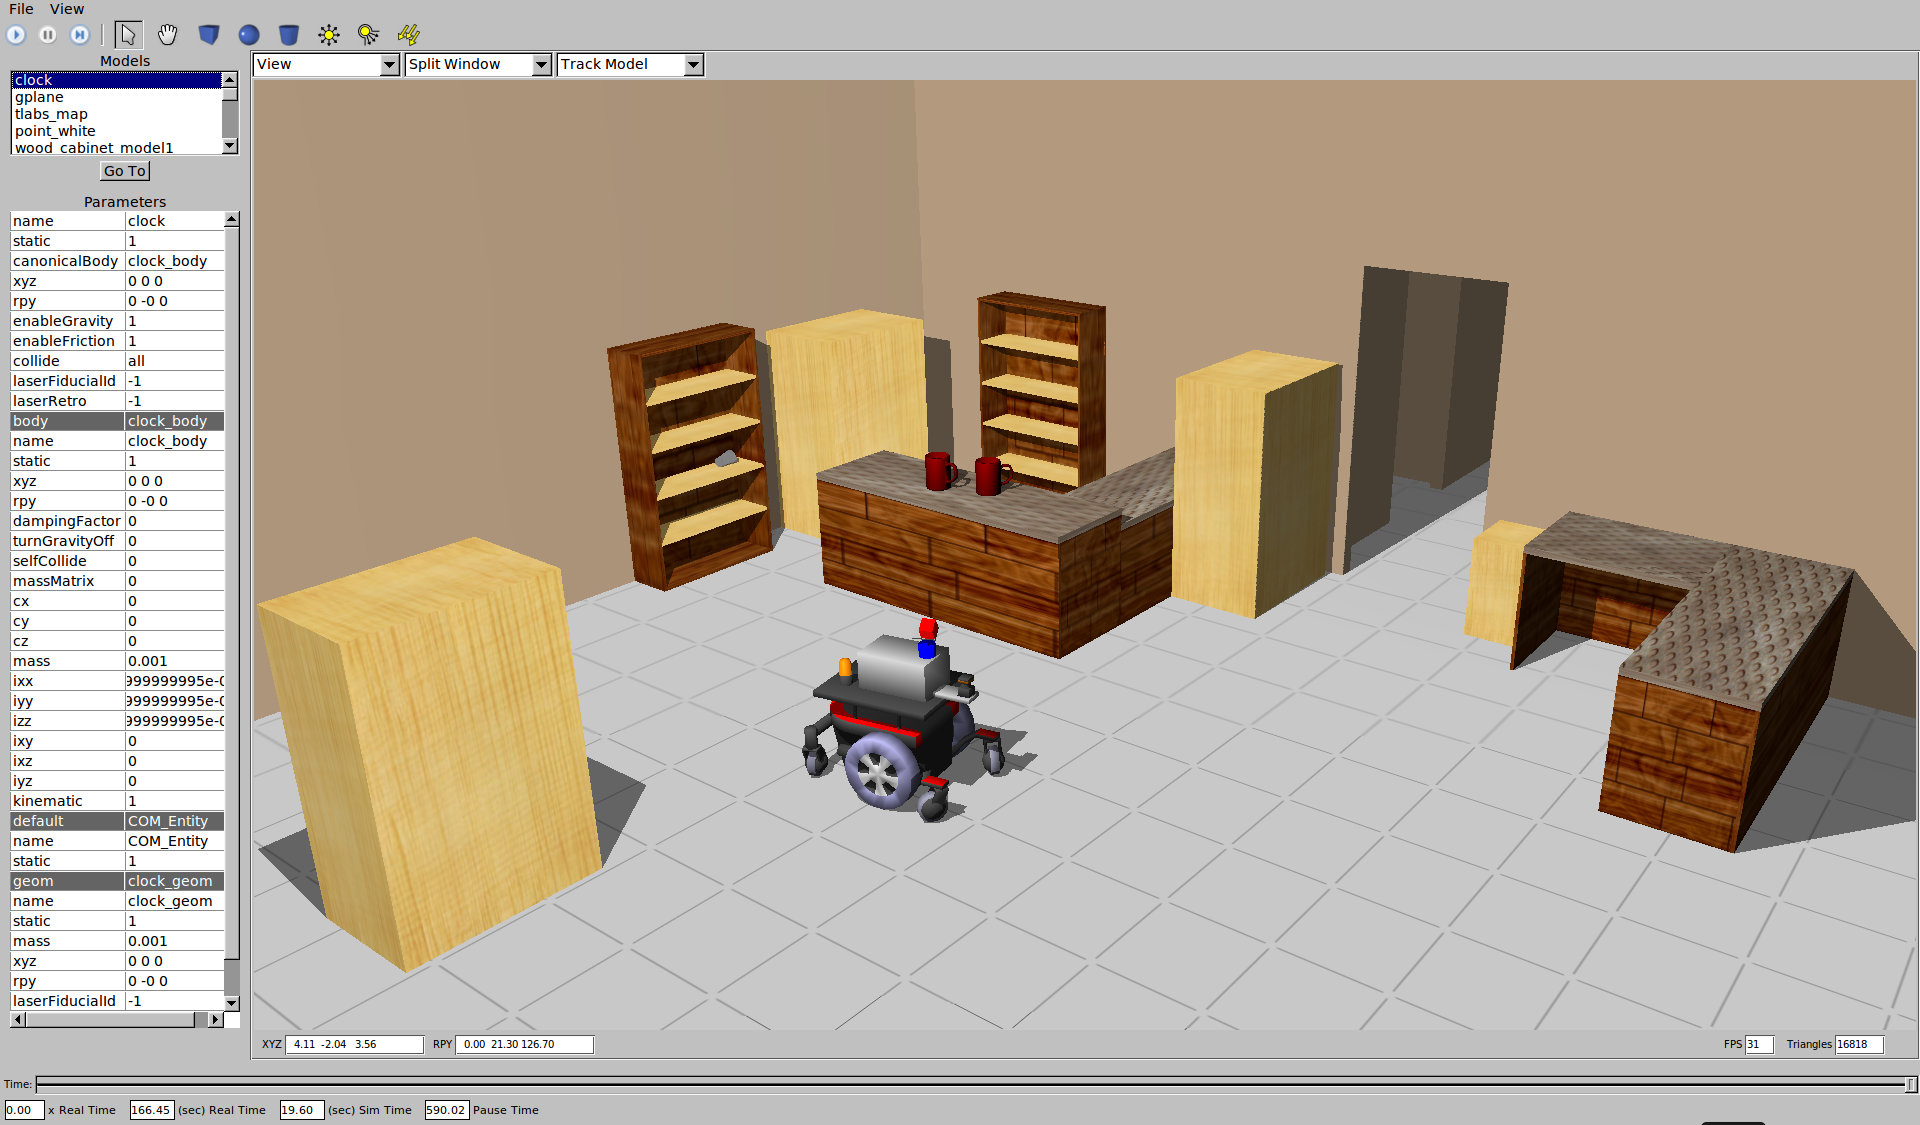
\includegraphics[width=1\linewidth]{image/gazebo_world.png}
      \caption{An example world in Gazebo}
      \label{fig:gazebo_world}
  \end{figure}
  
  \newpage
  \item \textbf{Model file}: This file shares the same format SDF with world files. However, it includes only one model (may be a robot) each file:
  \begin{lstlisting}
  <model>
   ...
  </model>
  \end{lstlisting}
  Using these model files, you can insert a model into many worlds, without the need to re-write it. It also simplifies the structure of a world file, because instead of pasting the whole robot structure, you just need 3 simple lines of code:
  \begin{lstlisting}
  <include>
    <uri>model://model_file_name</uri>
  </include>
  \end{lstlisting}
  Many sample models are available to be downloaded on\\ https://bitbucket.org/osrf/gazebo\_models. You can also make a custom model. This problem will be discussed in the next part.
  \item \textbf{Environment variables}: These variables in Gazebo can be thought about as global variables. They are used to locate files and setup communications between the server and clients.\\
  Gazebo offers a list of default values for these variables, included in a shell script. You should always run this script before making any modification to Gazebo:
  \begin{lstlisting}
  source usr/share/gazebo-2.2/setup.sh
  \end{lstlisting}
  \item \textbf{Gazebo server}: gzserver is a headless running (no GUI) executable, which can be referred to as the most important. It parses a world file and simulates that world with its physics update-loop and sensor data generation. It's the core of Gazebo, and can as well run on a cloud server, providing most basic needs for other clients.\\
  Gazebo server can be called upon a world by command:
  \begin{lstlisting}
  gzserver <world_filename>
  \end{lstlisting}
  
  \newpage
  world\_filename can be:
  \begin{enumerate}
  \item An absolute path.
  \item A relative path to current directory.
  \item relative to a path component in GAZEBO\_RESOURCE\_PATH.
  \end{enumerate}
  \item \textbf{Graphical client}: gzclient runs a QT-based GUI to visualize the work of gzserver. It also provides tools to modify the running simulation, its properties and plugins.\\
  You can call Graphical client while a gzserver has been already running. Open another Terminal and enter:
  \begin{lstlisting}
  gzclient
  \end{lstlisting}
  You should see the Gazebo GUI now.\\
  You can also run both server and client by using the command:
  \begin{lstlisting}
  gazebo <world_filename>
  \end{lstlisting}
  However, restarting gzclient is faster than gzserver. If you start server and client separately, you can also run multiple interfaces (Gazebo windows) at once.
  \begin{figure}[h]
      \centering
      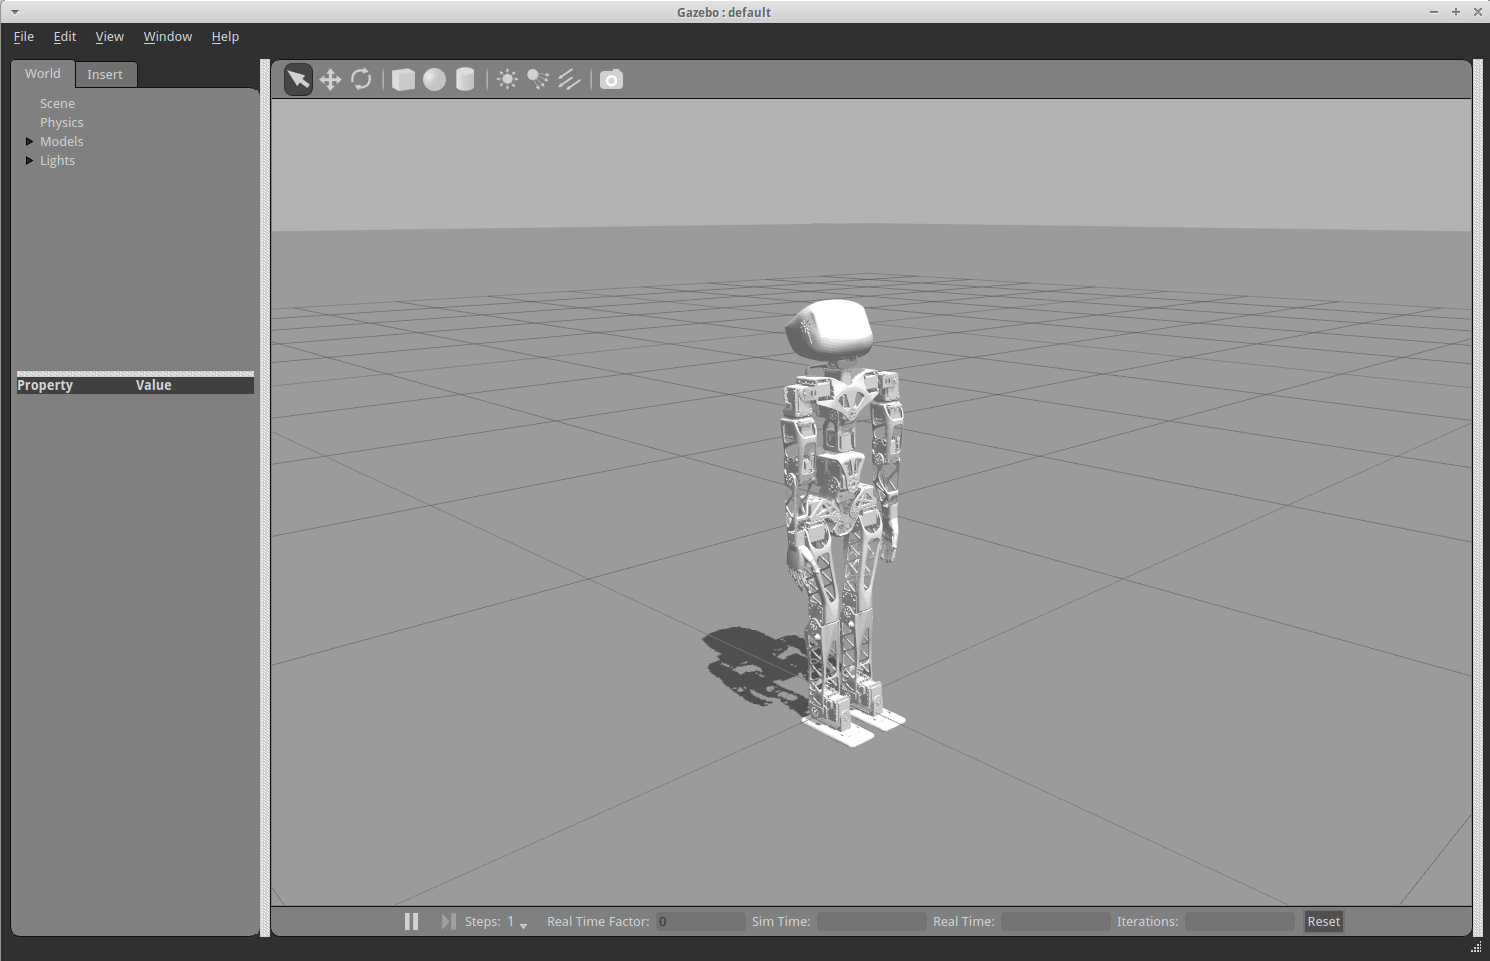
\includegraphics[width=0.9\linewidth]{image/gazebo_default.png}
      \caption{The default interface of Gazebo}
      \label{fig:gazebo_default}
  \end{figure}
  
  \end{itemize}
  
  \lstset{language=XML,
    keywordstyle=\color{ProcessBlue},
    keywordstyle=[2]\color{OliveGreen},
    keywordstyle=[3]\color{Fuchsia},
    commentstyle=\color{Blue},
    stringstyle=\color{red},
    morekeywords={
    	include, pr2\_wheel,
    	geometry,origin, circle,
    	link, collision, box, inertial,
    	mass
    },
    morekeywords=[2]{
    	name, value, type, radius, length,
    	xyz, rpy, circumference, filename,
    	size, ixx, ixy, ixz, iyy, iyz, izz
    },
    morekeywords=[3]{
     	xacro:property, xacro:insert\_block,
     	xacro:include,
     	robot
    }
  }
  
  \newpage
  \subsubsection{Xacro file structure}
  A Gazebo model is often written in SDF, as mentioned above. However, for this project, mutual work between ROS and Gazebo making SDF a bad option, for ROS can hardly work with a .sdf file (many work-around and errors). Therefore, I used another format for the modeling: \textbf{xacro}.\\
  Xacro (XML Macros) is a macro language, which can be used to construct shorter and more readable XML files. ROS have full support for xacro with the "xacro" package, and Gazebo can work with that package to simulate the robot.\\
  Similar to SDF, a XACRO robots are made of Links, Joints, and optionally Plugins.
  \begin{itemize}
  \item \textbf{Links} stores physical properties of a part of the model. These properties include elements like "collision", "visual", "inertial" and "sensor".\\
  Collision encapsulates a geometry that is used for collision checking. A link may have many collisions.\\
  Visual visualizes parts of a link. You can choose to have no visual, then the displayed part will be the geometry shape of the collision. Visual is used to import meshes (that you designed in another program) to the model in simulation.\\
  Inertial describes the dynamic properties of the link, such as mass and rotational inertia matrix. A robot body should have a large inertial to prevent shaking in simulation.\\
  Sensor collects data from the virtual world and use them in plugins.
  \item \textbf{Joints} connect links. A parent and child relationship is established along with other parameters such as axis of rotation, and joint limits.
  \item \textbf{Plugins} are shared libraries to control a model.
  \end{itemize}
  Therefore, to make a model, you must ensure that all those parameters in the xacro file has been defined appropriately.
  
  \newpage
  In addition, xacro files may contain their own Properties.\\
  \textbf{Properties} are named values that can be inserted anywhere into the XML document. It works just like a variable in C. For example, one want to make a "the\_radius" variable, and use it in a cylinder geometry:
  \begin{lstlisting}
    <xacro:property name="the_radius" value="2.1" />
    <xacro:property name="the_length" value="4.5" />
    
    <geometry type="cylinder" radius="${the_radius}" length="${the_length}" />
  \end{lstlisting}
  Properties are inserted into the geometry expression by placing the names inside dollared-braces (\$\{\}). If you want a literal "\$\{", you should escape it as "\$\$\{".\\
  Aside from Properties, one can also define a Property Block. The block is used when you want to pre-define a complex block of code, which can be repeated many times in your model. Here is an example:
  \begin{lstlisting}
    <xacro:property name="front_left_origin">
      <origin xyz="0.3 0 0" rpy="0 0 0" />
    </xacro:property>
    
    <pr2_wheel name="front_left_wheel">
      <xacro:insert_block name="front_left_origin" />
    </pr2_wheel>
  \end{lstlisting}
  Within dollared-braces (\$\{\}), you can also write simple math expressions. Currently, basic arithmetic and variable substitution is supported. Here's an example: 
  \begin{lstlisting}
    <xacro:property name="pi" value="3.1415926535897931" />
    <circle circumference="${2.5 * pi}" />
  \end{lstlisting}
  And finally, you can also include other xacro files inside one.
  \begin{lstlisting}
    <xacro:include filename="other_file.xacro" />
  \end{lstlisting}
  
  \newpage
  \subsubsection{Write xacro file for robot}
  In this project, the goal is to create and simulate a robot arm. It would be a good idea to plan a sequence in creating one. I would choose this order, suggested by Gazebo:
  \begin{enumerate}
  \item Sketch the overall look of the arm.
  \item Add a link.
  \item Set the collision element.
  \item Set the inertial properties.
  \item Go to \#2 until all links have been added.
  \item Add all joints (if any)
  \item Add visual meshes (will be done later in the next parts)
  \end{enumerate}
  So the first part is to sketch an abstract image of the arm:
  \begin{figure}[h]
      \centering
      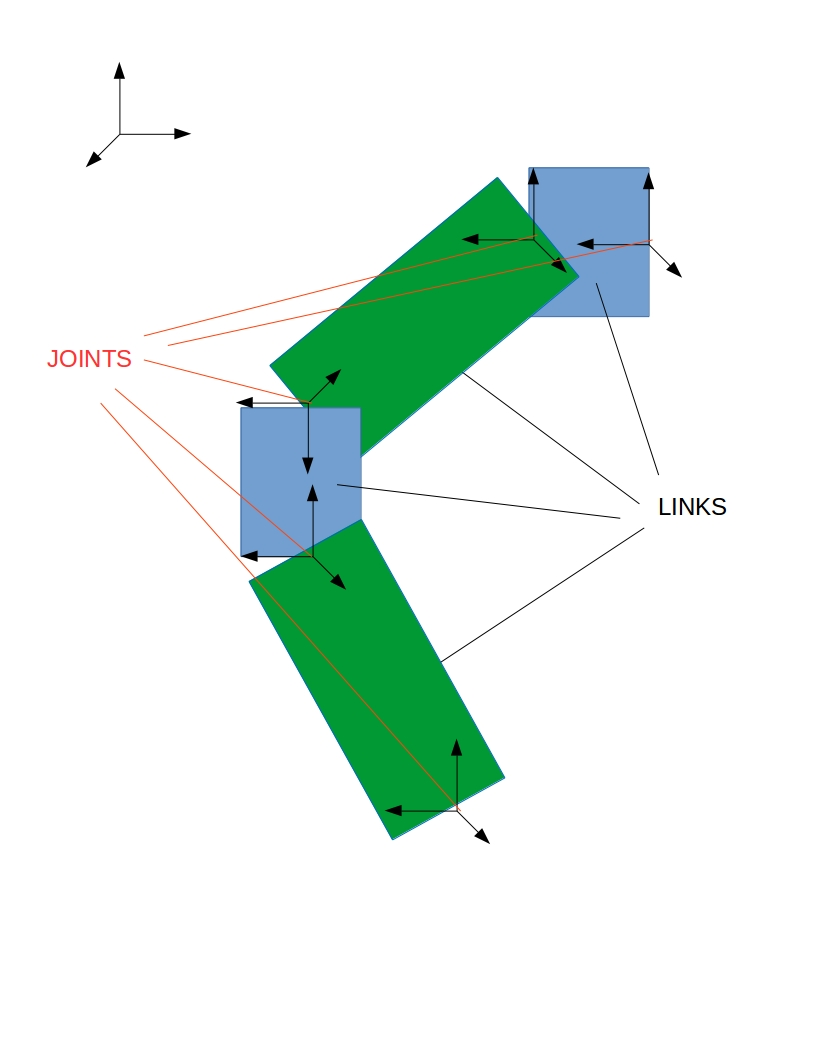
\includegraphics[width=0.5\linewidth]{image/gazebo_links.jpg}
      \caption{The arm model with links and joints}
      \label{fig:arm_links}
  \end{figure}
  
  \newpage
  As we can see, the model consists of 4 links and 5 joints.\\
  Next 3 steps is to add the first link with its collision and inertial elements:
  \begin{lstlisting}
    <?xml version="1.0"?>
    <robot name="arm" xmlns:xacro="http://www.ros.org/wiki/xacro">
    
    <!-- First Link -->
    <link name="shoulder">
      <collision>
          <origin xyz="0 0 ${height1/2}" rpy="0 0 0"/>
          <geometry>
    	    <box size="${width} ${width} ${height1}"/>
          </geometry>
      </collision>
    
      <inertial>
          <origin xyz="0 0 ${height1/2}" rpy="0 0 0"/>
          <mass value="1000"/>
          <inertia
    	  ixx="0.10" ixy="0.0" ixz="0.0"
    	  iyy="0.10" iyz="0.0"
    	  izz="0.10"/>
      </inertial>
    </link>
  \end{lstlisting}
  The first link is named "link1". Creating other 3 links with following names would complete our first part of making links:
  \begin{lstlisting}
    <link name="shoulder">
      ...
    </link>
    
    <link name="arm">
      ...
    </link>
    
    <link name="elbow">
      ...
    </link>
    
    <link name="forearm">
      ...
    </link>
  \end{lstlisting}
  
  \newpage
  It's also worth time to explain some parameters inside the <link> block.
  \begin{itemize}
  \item name: This should explain itself, but remember to name the links as easy to remember as possible, make it short and descriptive. Avoid names like "a" or "the\_link\_which\_is\_long\_and\_complex".
  \item xyz: the relative position of the link, with respect the previous link.
  \item rpy: rotating angle of the link.
  \item box size: create a box with x, y, z dimensions respectively as written. You can change this "box" into "cylinder" or other geometry shapes of Gazebo.
  \item ixy: XY inertia
  \item ixx: X second moment of inertia (MOI) about x axis.
  \end{itemize}
  Here's an image of my model (with 2 arms already) containing the links (shown as basic shapes/ boxes).
  \begin{figure}[h]
      \centering
      
\includegraphics[width=0.5\linewidth]{image/FH-Frankfurt.jpg}
      \caption{The dual arm model in Gazebo with links shown}
      \label{fig:arm_gazebo_link}
  \end{figure}
  
  \newpage
  Note: To insert a model into Gazebo, simple solution is to move the model to one of Gazebo default paths and use Insert in Gazebo GUI.
  \begin{figure}[h]
      \centering
      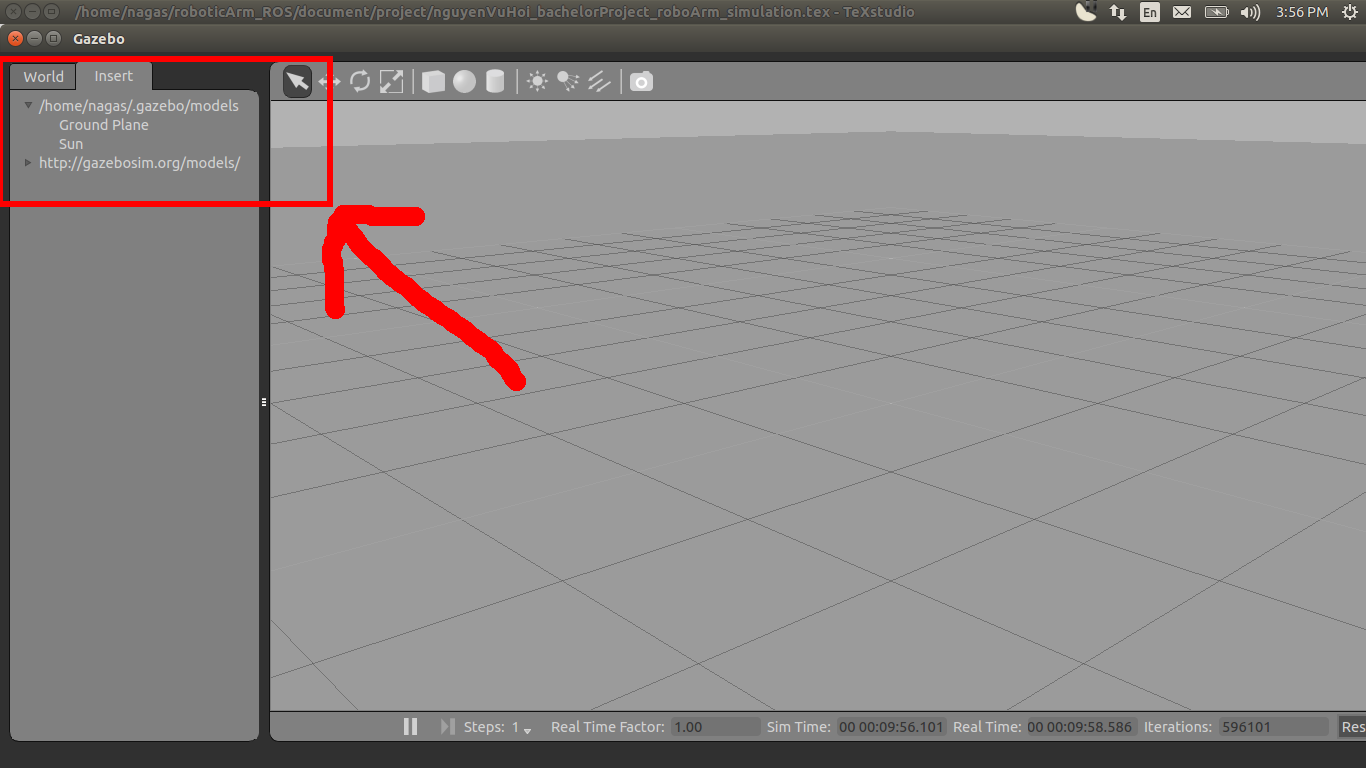
\includegraphics[width=0.9\linewidth]{image/gazebo_insert.png}
      \caption{Click a model in Insert tab to spawn them to the world}
      \label{fig:gazebo_insert}
  \end{figure}\\
  Next step is to make joints between links.\\
  Firstly, if you want to fix your arm to the world, so that it can move as expected, a default "world" link should be called and the first joint should connect "world" to your first link. In this situation, I made a "dummy body" link, called "base\_link". That body will stick to the "world" link at one end, and the "should" link at the other. As the base\_link is quite similar to other link, re-write it here may cost useless space, so I assume it has been made. First, let's make the "world" link:
  \begin{lstlisting}
    <!-- world_link, used for fixing robot to Gazebo base_link -->
    <link name="world"/>
  
    <!-- Connect with dummy body to hold the arms -->
    <joint name="fixed" type="fixed">
    
      <parent link="world"/>
      <child link="base_link"/>
    </joint>
  \end{lstlisting}
  
  \newpage
  It's that simple. Now, let's make the joint between the shoulder and the arm.
  \begin{lstlisting}
    <joint name="joint1_1" type="continuous">
    
      <parent link="shoulder"/>
      <child link="arm"/>
      
      <origin xyz="0 ${elbow_width/2+0.04} ${-elbow_width*0}" rpy="0 0 0"/>
      <axis xyz="1 0 0"/>
      <dynamics damping="0.7"/>
    </joint>
  \end{lstlisting}
  Repeat this structure for other joints, and name them joint1\_2, joint2\_1, joint2\_2, joint3\_1.\\
  This should finish the modeling of the robot arm for Gazebo on xacro file.\\
  Below is the arms with joints displayed.
  \begin{figure}[h]
      \centering
      
\includegraphics[width=0.5\linewidth]{image/FH-Frankfurt.jpg}
      \caption{Joints in dual arm model}
      \label{fig:arm_gazebo_joint}
  \end{figure}
  
  \newpage
  \subsubsection{Arm design}
  An arm is designed and assembled in another CAD software. The requirements are that there is always an equivalent part for each link in the xacro model:
  \begin{itemize}
  \item A round shoulder as "shoulder" link. This part has a metal plate to be easily connected to the dummy body.
  \item A quite big arm, resembling human arm, as "arm" link.
  \item An elbow, which is not quite visible in the next image. For better appearance purpose, an elbow-cover part is added.
  \item The last link should be the forearm and the hand, as I don't want to control the hand, I just designed a good-looking static hand.
  \end{itemize}
  Here is the rendered image of the arm:
  \begin{figure}[h]
      \centering
      \includegraphics[width=0.9\linewidth]{image/arm_brushedmetal.JPG}
      \caption{Rendered brushed metal arm}
      \label{fig:arm_gazebo_rendered}
  \end{figure}
  
  \newpage
  \subsubsection{Import meshes}
  Inside the CAD program, you should \textbf{prepare the mesh}. The mesh is a solid body of separate parts (four parts in my design), imported as a .stl file for working with Gazebo.\\
  First thing to do is centering the mesh at (0,0,0) and orient the front (which can be subjective) along the x-axis..\\
  Next, scale the mesh to metric system, as that is the unit system in Gazebo.\\
  Last thing is to reduce the complexity of the mesh. This helps simulate faster, without having the trade off too much quality of the image. Use the options in the 3D CAD to reduce the number of triangles count.\par
  To \textbf{test the mesh}, one can make a simple file test.world to load the mesh. Here is the source code of the file, replacing [mesh\_path] with the path to your mesh:
  \begin{lstlisting}
  <?xml version="1.0"?>
  <sdf version="1.4">
    <world name="default">
      <include>
        <uri>model://ground_plane</uri>
      </include>
      <include>
        <uri>model://sun</uri>
      </include>
      <model name="my_mesh">
        <pose>0 0 0  0 0 0</pose>
        <static>true</static>
        <link name="body">
          <visual name="visual">
            <geometry>
              <mesh><uri>[mesh_path]</uri></mesh>
            </geometry>
          </visual>
        </link>
      </model>
    </world>
  </sdf>
  \end{lstlisting}
  Then use Gazebo to open the file. Your mesh should be visible.
  \begin{lstlisting}
  gazebo test.world
  \end{lstlisting}
  
  \newpage
  To \textbf{attach the mesh} to your model to add realism, you must define a link in the "visual" block of your macro file.\\
  \begin{lstlisting}
  <link name="shoulder">
  ...
  
    <visual>
    
      <origin xyz="1.1 -3.15 8" rpy="-1.57 0 1.57"/>
      <geometry>
    	<mesh   filename="package://arm_description/meshes/shoulder.STL" scale="${scale+0.1} ${scale+0.1} ${scale+0.1}"/>
      </geometry>
    </visual>
    ...
  </link>
  \end{lstlisting}
  As shown above, the mesh can be scaled, moved and rotated just like the collision. Copy and modify the code above to all links. Here is the model with meshes attached.
  \begin{figure}[h]
      \centering
      
\includegraphics[width=0.6\linewidth]{image/FH-Frankfurt.jpg}
      \caption{Dual arm model with meshes}
      \label{fig:arm_gazebo_mesh}
  \end{figure}
  
  \newpage
  \subsubsection{Make a launch file}
  A launch file is like a macro file for Gazebo. It load the world with ability to pre-configure the arguments. Because it is impossible to insert directly a xacro model to Gazebo, a launch file can use an indirect python script to generate files needed for the package gazebo\_ros to spawn the model into the mentioned world. Create arm\_world.launch file with this code:
  \begin{lstlisting}
  <launch>
    <!-- pre-configurable variable -->
    <arg name="paused" default="false"/>
    <arg name="use_sim_time" default="true"/>
    <arg name="gui" default="true"/>
    <arg name="headless" default="false"/>
    <arg name="debug" default="false"/>
  
    <include file="$(find gazebo_ros)/launch/empty_world.launch">
      <arg name="world_name" value="$(find arm_gazebo)/worlds/arm.world"/>
      <arg name="debug" value="$(arg debug)" />
      <arg name="gui" value="$(arg gui)" />
      <arg name="paused" value="$(arg paused)"/>
      <arg name="use_sim_time" value="$(arg use_sim_time)"/>
      <arg name="headless" value="$(arg headless)"/>
    </include>
  
    <!-- Load the XACRO into the ROS Parameter Server -->
    <param name="robot_description"
  	 command="$(find xacro)/xacro.py '$(find arm_description)/urdf/arm.xacro'" />
  
    <!-- Run a python script to the send a service call to gazebo_ros to spawn a URDF robot -->
    <node name="urdf_spawner" pkg="gazebo_ros" type="spawn_model" respawn="false" output="screen"
  	args="-urdf -model arm -param robot_description"/>
  </launch>
  \end{lstlisting}
  Then calling the launch file will use Gazebo to open the file.
  \begin{lstlisting}
  roslaunch arm_world.launch
  \end{lstlisting}
  
  \newpage
  \subsubsection{Applying force/torque}
  Let's open Gazebo and insert the arm into it (using roslaunch)with the simulation not paused.\\
  In the World tab, right click on a link to apply force/torque. Then choose the force or torque, its axis, and click Apply. The force is applied in a millisecond, so if the arm is to move noticeably, a large amount (about 100N) should be entered.\\
  Note that "Mag" is the total magnitude of the force which will be applied, which is the Euclidean norm of the 3 forces.
  \begin{figure}[h]
      \centering
      
\includegraphics[width=0.6\linewidth]{image/FH-Frankfurt.jpg}
      \caption{Apply force/torque to links}
      \label{fig:arm_gazebo_applyForce}
  \end{figure}
  
  \newpage
  \subsection{Control Gazebo by ROS}
  As we can see from the previous section (Gazebo Simulation), Gazebo can apply forces to move the links. However, to really control the joints, we need something like ROS. This doesn't only help controlling accurately with message-based communication, but also give a chance to synchronize between simulation and real-time system. This can be helpful can save much time if one wants to expand this project in the future.
  \subsubsection{Overview about ROS-Gazebo relationship}
  In this part we will not talk about the history between two software packages, but the relationship between simulation, hardware, controllers and transmissions. Firstly, let's take a look at how ROS works with real-life hardware.
  \begin{figure}[h]
      \centering
      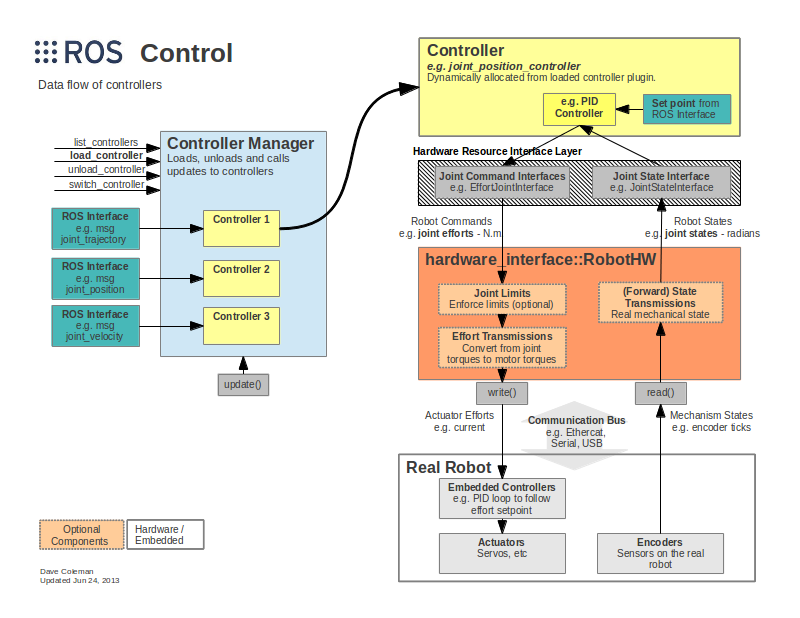
\includegraphics[width=0.9\linewidth]{image/gazebo_ros_control.png}
      \caption{ROS control in relationship with a real robot}
      \label{fig:gazebo_ros_control}
  \end{figure}
  
  \newpage
  As suggested in the Figure \ref{fig:gazebo_ros_control}, a controller receives messages from the Controller Manager of ROS, sending controlling signals to the hardware interface (for example Arduino). This hardware will directly move the robot, read feedback and transfer back to the controller. This works as a loop can continuously give commands to the robot, according to written software.\\
  Controller Manager manages many controllers and consecutively update both the user commands to hardware and feedback information to users.\\
  Now that we can somehow imagine how "real-time" ROS works, we can make a comparison between the "virtual" and "real" system.
  \begin{figure}[h]
      \centering
      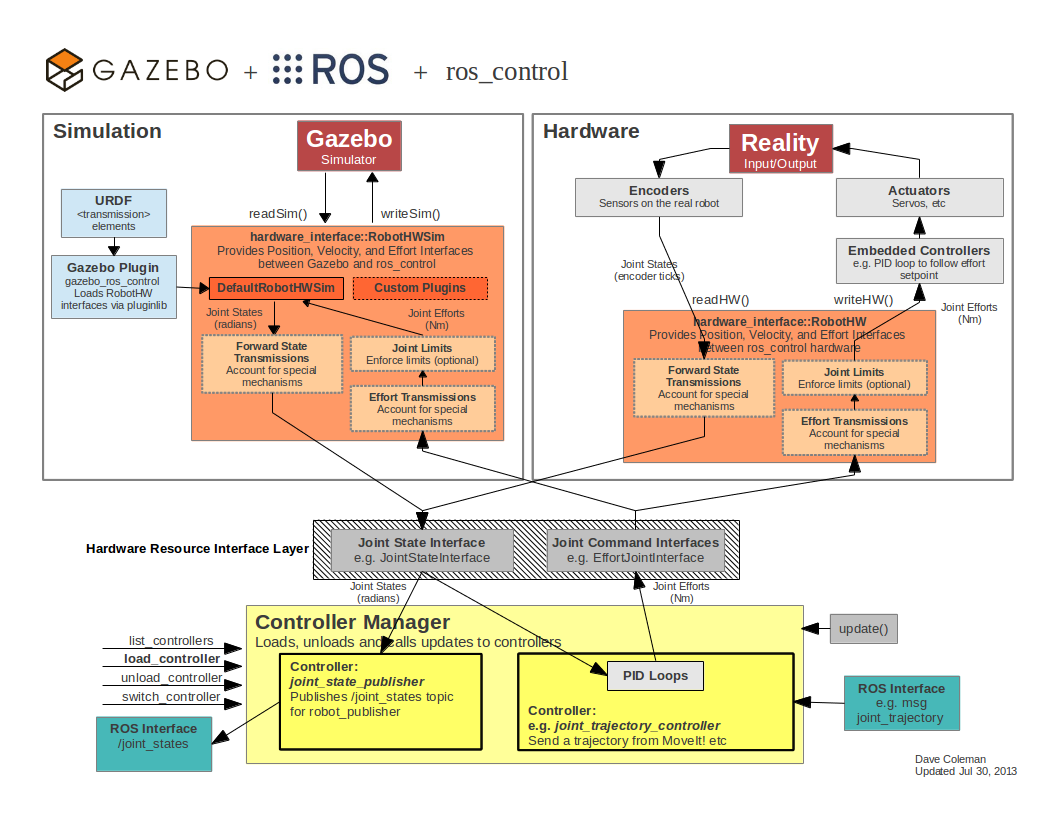
\includegraphics[width=0.9\linewidth]{image/Gazebo_ros_transmission.png}
      \caption{ROS control in Gazebo vs. Reality}
      \label{fig:gazebo_ros_transmission}
  \end{figure}
  Here we can see, there are not many differences between 2 systems. The hardware interface is quite similar, apart from the plugins and the default simulated robot hardware. The physics engine of Gazebo has the role to imitate the behavior of real hardware components in a real electrical system.
  
  \newpage
  \subsubsection{Add transmission element}
  To control the Gazebo joints, there need to be a "virtual actuator". The transmission element is used for that purpose, linking one joint to one actuator. Add this block of code to the xacro file, inside the "robot" element:
  \begin{lstlisting}
    <transmission name="trans_joint1_1">
      <type>transmission_interface/SimpleTransmission</type>
      <joint name="joint1_1">
        <hardwareInterface>EffortJointInterface</hardwareInterface>
      </joint>
      <actuator name="motor1_1">
        <hardwareInterface>EffortJointInterface</hardwareInterface>
        <mechanicalReduction>1</mechanicalReduction>
      </actuator>
    </transmission>
  \end{lstlisting}
  The "name" attribute must be unique. The basic elements are:
  \begin{itemize}
  \item \textbf{type}: transmission\_interface/SimpleTransmission. Define the type of this transmission element as Simple Reduction Transmission. A transmission can only have 1 type.
  \item \textbf{joint}: The joint name the transmission is connected to. A transmission can have 1 or more joints. "HardwareInterface" specifies a supported joint-space hardware interface.
  \item  \textbf{actuator}: The actuator name the transmission is connected to. A transmission can have 1 or more actuators. "mechanicalReduction" element specifies a mechanical reduction at the joint/actuator transmission. It is optional.
  \end{itemize}
  Recursively make transmissions for other joints. These virtual actuators, though have been defined, can yet been used. It needs more configurations to be able to work.
  
  \newpage
  \subsubsection{Add gazebo\_ros\_control plugin}
  At the upper left corner of Figure \ref{fig:gazebo_ros_transmission}, it's shown that Gazebo needs a Gazebo plugin named gazebo\_ros\_control. Since we replaced URDF file format with XACRO, we need to modify the xacro file to include that plugin.\\
  To do that, we need a "gazebo" element to contain those modifications:
  \begin{lstlisting}
  <gazebo>
    (everything related to gazebo plugin comes here)
  </gazebo>
  \end{lstlisting}
  For the simplification of the code, and the ability to use nested files of XACRO, I made another arm.gazebo file inside the same directory as arm.xacro to contain all gazebo-related codes.\\
  Open arm.gazebo and add these lines:
  \begin{lstlisting}
  <?xml version="1.0"?>
  <robot>
  
    <!-- ros_control plugin -->
    <gazebo>
      <plugin name="gazebo_ros_control" filename="libgazebo_ros_control.so">
        <robotNamespace>/arm</robotNamespace>
        <robotSimType>gazebo_ros_control/DefaultRobotHWSim</robotSimType>
      </plugin>
    </gazebo>
  </robot>
  \end{lstlisting}
  The gazebo\_ros\_control plugin has the following optional elements:
  \begin{itemize}
  \item \textbf{robotNamespace}: The ROS namespace to be used for this instance of the plugin, defaults to robot name in URDF/SDF/XACRO
  \item \textbf{controlPeriod}: The period of the controller update (in seconds), defaults to Gazebo's period
  \item \textbf{robotParam}: The location of the arm\_description (URDF) on the parameter server, defaults to '/arm\_description'
  \item \textbf{robotSimType}: The pluginlib name of a custom robot sim interface to be used, defaults to 'DefaultRobotHWSim'
  \end{itemize}
  
  \newpage
  \subsubsection{Create arm\_control package}
  As the arm\_description with xacro files have been configured and ready, what's left is just how we should control them.\\
  Let's start with saving controller settings into a yaml file. Create a package named arm\_control and make a folder named "config":
  \begin{lstlisting}
  catkin_create_pkg MYROBOT_control ros_control ros_controllers
  cd MYROBOT_control
  mkdir config
  \end{lstlisting}
  Navigate to the "config" folder, create arm\_control.yaml file with this content (fill the "..." with similar information):
  \begin{lstlisting}
  arm:
    # Publish all joint states -----------------------------------
    joint_state_controller:
      type: joint_state_controller/JointStateController
      publish_rate: 50
      
    # Position Controllers ---------------------------------------
    joint1_1_controller:
      type: effort_controllers/JointPositionController
      joint: elbow1_1
      pid: {p: 130.0, i: 60.00, d: 60.0}
    joint1_2_controller:
      ...
    joint2_1_controller:
      ...
    joint2_2_controller:
      ...
    joint3_1_controller:
      ...
  \end{lstlisting}
  Then I tuned the PID control to work well with my robot.
  
  \newpage
  Next, to make working with ros\_control an ease, a launch file should be made. If the launch file in arm\_gazebo is to create world and spawn model, this launch file load the configurations in yaml file, load the controllers and convert joint states to TF transform.\\
  Create a file arm\_control.launch in arm\_control package's launch directory and add this code:
  \begin{lstlisting}
  <launch>
  
    <!-- Load joint controller configurations from YAML file to parameter server -->
    <rosparam file="$(find arm_control)/config/arm_control.yaml" command="load"/>
  
    <!-- Controller Manager >
    <include file="$(find pr2_controller_manager)/controller_manager.launch" /-->
  
    <!-- load the controllers -->
    <node name="controller_spawner" pkg="controller_manager" type="spawner" respawn="false"
  	output="screen" ns="/arm" args="joint1_1_controller joint1_2_controller joint2_1_controller joint2_2_controller joint3_1_controller "/>
  
    <!-- convert joint states to TF transforms for rviz, etc -->
    <node name="robot_state_publisher" pkg="robot_state_publisher" type="robot_state_publisher"
  	respawn="false" output="screen">
      <remap from="/joint_states" to="/arm/joint_states" />
    </node>
  </launch>
  \end{lstlisting}
  Everything is alright now. Go to the catkin\_ws and run:
  \begin{lstlisting}
  catkin_make
  \end{lstlisting}
  This builds all your packages. If no error occurs, the project is ready to run.
  
  \newpage
  \subsubsection{Start controllers and manually send commands}
  Now we can test the robot. First, simulate the world and spawn the robot, using the written launch file in arm\_gazebo package:
  \begin{lstlisting}
  roslaunch arm_gazebo arm_world.launch
  \end{lstlisting}
  Open another Terminal and run the controllers.
  \begin{lstlisting}
  roslaunch arm_control arm_control.launch
  \end{lstlisting}
  Now the environment has been set. One can check the controllers:
  \begin{lstlisting}
  rosservice list
  \end{lstlisting}
  Stop the controllers:
  \begin{lstlisting}
  rosservice call /arm_control/controller_manager/switch_controller "{start_controllers: [], stop_controllers: ['joint1_1_controller'], strictness: 2}"
  \end{lstlisting}
  Or start it:
  \begin{lstlisting}
  rosservice call /arm_control/controller_manager/switch_controller "{start_controllers: ['joint1_1_controller'], stop_controllers: [], strictness: 2}"
  \end{lstlisting}
  And you can manually send commands to joints:
  \begin{lstlisting}
  rostopic pub -1 /arm_control/joint1_1_controller/command std_msgs/Float64 "data: 1.57"
  \end{lstlisting}
  
  \newpage
  \subsubsection{Use RQT to send commands}
  RQT is a ROS plugin-based UI, a simple tool to visualize the performance of controllers. AFter already running roscore, RQT can be started by:
  \begin{lstlisting}
  rosrun rqt_gui rqt_gui
  \end{lstlisting}
  To publish a command to a topic, on the 'Plugins' menu of RQT add the 'Topics/Message Publisher' plugin. Then choose the topic from the drop down box. For example:
  \begin{lstlisting}
  /arm_control/joint1_1_controller/command
  \end{lstlisting}
  And press the green button. Set the "rate" column to 100 (frequency to send command, 100Hz). In "data" row, try different values to control the joint. For example, a sine wave:
  \begin{lstlisting}
  sin(i/100)
  \end{lstlisting}
  A more advanced version:
  \begin{lstlisting}
  sin(i/rate*speed)*diff + offset
  \end{lstlisting}
  With:\\
  \begin{itemize}
  \item i - the RQT variable for time
  \item rate - the frequency that this expression is evaluated. This should be the same number as in the rate column of the topic publisher. Recommended value is 100.
  \item speed - how quick you want the join to actuate. Start off with just 1 for a slow speed
  \item upper\_limit and lower\_limits - the joint limits of the hardware being controlled by this controller
  \item diff = (upper\_limit - lower\_limit)/2
  \item offset = upper\_limit-diff
  \end{itemize}
  
  \newpage
  \subsubsection{Use SQT to visualize controller's performance}
  Add the "Plot" plugin to RQT. Choose the same topic as chosen in Message Publisher Plugin.
  \begin{lstlisting}
  /arm_control/joint1_1_controller/command/data
  \end{lstlisting}
  Click the green add button, that displays a sine wave being plotted on the screen.\\
  Add another topic to the Plot plugin that tracks the error between the commanded position and actual position of the actuator being controlled.
  \begin{lstlisting}
  /arm_control/joint1_1_controller/state/process_value
  \end{lstlisting}
  If things get strange after a while running Plot plugin, click the blue refresh button at the top right of the plugin.\\
  The result of above experiment should look like this:
  \begin{figure}[h]
      \centering
      
\includegraphics[width=0.6\linewidth]{image/FH-Frankfurt.jpg}
      \caption{Comparison between controlling signal and actual position.}
      \label{fig:gazebo_rqt}
  \end{figure}
  
  \newpage
  \subsection{Project studying timeline}
  I signed to start the project at 04 May, 2015. The project lasts 4 weeks, so the deadline is in 01/06. Follow is my schedule for parts:
  \begin{itemize}
  \item 04/05 - 08/05: Installation needed software, including Ubuntu, ROS Indigo, Gazebo 2, plugins.
  \item 08/05 - 14/05: Study ROS, including doing tutorials, reading package information, asking for experience, experiment sending (publishing) and receiving (subscribing) custom messages.
  \item 14/05 - 19/05: Study Gazebo, including doing tutorials, code my arm's xml files, running launch files and use built-in force applying of Gazebo.
  \item 19/05 - 23/05: Design the arm on CAD program and import the meshes into Gazebo.
  \item 23/05 - 28/05: Use gazebo\_ros\_control plugin to control the arm inside Gazebo, using ROS communicating style.
  \item 25/05 - 31/05: Learn LaTeX, write report and summarize the project.
  \item 01/06: Due date of the project.
  \end{itemize}
  
  \newpage
  \section{Implementation}
  \subsection{A simple task of exercising}
  For the implementation part of this project, I will make the arms of the robot move, imitating the movement of humans while exercising. The result is shown below:
  \begin{figure}[h]
      \centering
      
\includegraphics[width=0.6\linewidth]{image/FH-Frankfurt.jpg}
      \caption{The arm moving its hands, like a simple exercise}
      \label{fig:arm_exercise}
  \end{figure}
    
  \newpage
  \section{Conclusion}
  The project has been completed fulfilling the initial goal. We can now control a model inside Gazebo either with messages published on a topic in ROS or by SQT GUI.\par
  We can simulate the robot in a virtual environment, knowing how it would move in real life if a command is given.\par
  The ROS structure and basic skills have been studied. It doesn't only promote my skill with working on Command Line Interface, but also provide a solid knowledge about the way to work with an infrastructure in Linux. The configurations and modeling based on files is an interesting topic to learn about.\par
  And finally, I could perform a simple implementation with the model in virtual world, proving the accurate controlling potential of this method.
  
  \newpage
  \section{Reference}
  \begin{enumerate}
  \item Introduction to Robotics: Mechanics and Control, John J. Craig, third edition, last retrieved 05/05/2015.
  \item The simplest ROS tutorial, http://jbohren.com/articles/roscpp-hello-world/, last retrieved 05/05/2015.
  \item A History of ROS, http://www.ros.org/history/, last retrieved 07/05/2015.
  \item ROS Indigo Tutorial, http://www.coppeliarobotics.com/helpFiles/en/rosTutorialIndigo.htm, last retrieved 09/05/2015.
  \item ROS tutorial on github, https://github.com/uscrs-art/uscrs-art/wiki, last retrieved 14/05/2015.
  \item ROS: an open-source Robot Operating System, VA, last retrieved 10/05/2015.
  \item ShareLaTeX guides, https://www.sharelatex.com/learn/, last retrieved 25/05/2015.\
  \item Linux is the platform for robotics, http://www.linuxuser.co.uk/features/linux-is-the-platform-for-robotics, last retrieved 25/05/2015.
  \item Gazebo Tutorials, http://gazebosim.org/tutorials, last retrieved 26/05/2015.
  \item LaTeX List Structures, http://en.wikibooks.org/wiki/LaTeX/List\_Structures, last retrieved 28/05/2015.
  \item ROS Tutorial, http://wiki.ros.org/ROS/Tutorials, last retrieved 29/05/2015.
  \end{enumerate}
  
\end{document}